\chapter{Basalt design}
The vending machine should be able to sell only one item at a time, not returning any money. Surplus will be left for next purchase. The price of an item is selected automatically when the user selects a product. The machine only accepts 1, 2 and 5 kr. The price of the selected item is displayed as a two-decimal-value on two seven-segment-displays as will the current sum-available-for-purchase. 

\begin{figure}[h!]
\centering
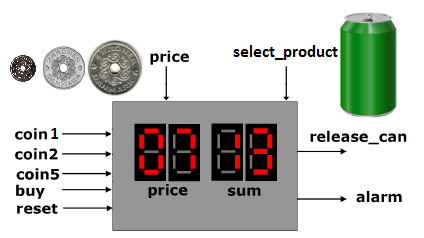
\includegraphics[scale=0.8]{figs/vendingdisplay.png}
\caption{Sketch of the vending machine}
\label{fig:vendingdisplay}
\end{figure}

As seen on figure \ref{fig:vendingdisplay} there is a number of user inputs. coin1, coin2, coin5 and buy is emulated by push-buttons on the FPGA board. The fifth 'input' select\_product, is emulated by switches, which choose between the different types of products, and the prices matching to every type. \\

When a product is chosen by a switch, the name of the product is shown for approximately 1.3 seconds. After this, the price is shown on the two digits to the left. The rightmost two digits represents the sum of the coins 'inserted' by the push-buttons coin1, coin2 and coin5. When the buy button is asserted, the price is subtracted from the sum if sum is greater than or equal to the price of the product. In the case where the sum is lower than the price, an alarm signal wlll be asserted, causing all four digits to blink for a fixed amount of time (approximately 1.3 seconds) on a 3Hz clock. If the 'Reset' switch is asserted, the sum is set to zero while the price of the products persists. \\

In designing the Vending Machine, we have created a number og VHDL entities, each controlling a part of the complete machine. Below is a block-diagram of our VHDL implementation of the machine. 

\begin{figure}[!h]
\centering
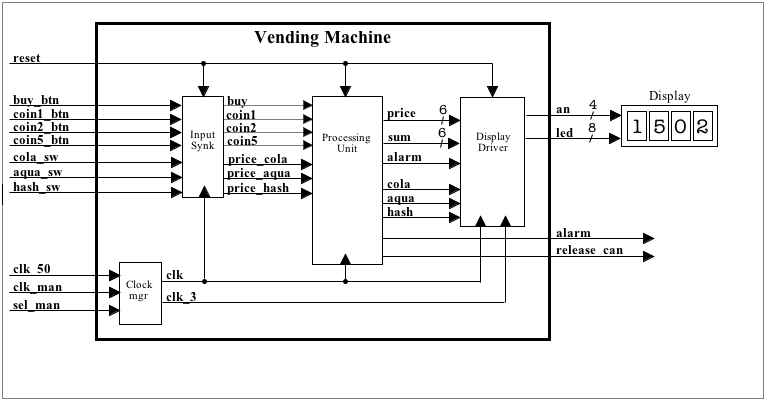
\includegraphics[scale=0.7]{figs/structure.png} 
\caption{The structure of our VHDL design, including the structure, entities and components}
\label{fig:structure}
\end{figure}